A system is judged by the quality of the services it offers and by its
ability to function reliably. Even though the reliability of operating
systems has been studied for several decades, it remains a major concern
today.

An analysis of the Linux kernel code conducted by Coverity in 2009 found
1000 bugs in the source code of version 2.4.1 of the Linux kernel and
950 bugs in version 2.6.9. This study also showed that 53\% of these bugs are
present in the device driver portions of the kernel~\cite{coveritykernel}.

In order to protect against bugs, operating systems provide protection
mechanisms. These protection mechanisms protect resources such as memory
and CPU.  Memory protection controls memory access rights. It prevents a
user process from accessing memory that has not been allocated to it. It
prevents a bug within a user process from affecting other processes
or the operating system~\cite{denning1970virtual, Galvin}. However,
kernel modules do not have the same level of protection user-level
applications have. In the Linux kernel, any portion of the kernel can
access and potentially overwrite kernel data structures used by unrelated
components. Such non-existent isolation between kernel components can
cause a bug in a device driver to corrupt memory used by other kernel
components, which in turn may lead to a system crash. Thus, a major underlying
cause of unreliability in operating systems is the lack of isolation
between device drivers and a Linux kernel.

\section {Problem Statement}
\label{sec:problem}
Virtualization based solutions to increase the reliability of a system were
proposed by LeVasseur et. al.~\cite{LeVasseur04UnmodifiedDriverReuse}
and Fraser et. al.~\cite{Fraser04safehardware,driverdomain}. Fraser et. al. proposed
isolated driver domains for the Xen hypervisor. In a virtualized
environment, virtual machines are unaware of and isolated from the other
virtual machines. Malfunctions in one virtual machine cannot spread to
the others, thus providing strong fault isolation.

In a virtualized environment, all virtual machines run as separate
guest domains in different address spaces. The virtualization based
solutions mentioned above exploit the memory protection facilities of these
guest domains. They improve the reliability of the system by executing
device drivers in separate virtual machines from the kernel. 
Isolated driver domains are based on the split
device driver model exploited by Xen~\cite{Chisnall:2007:DGX:1407351}.

Split device drivers are employed by Xen because its hypervisor
does not include device drivers,
instead it is relying on a dedicated, privileged guest domain to provide them.
Xen's split device driver model is shown in Figure~\ref{fig:xen-split}.
\begin{figure}[!ht]
\centering
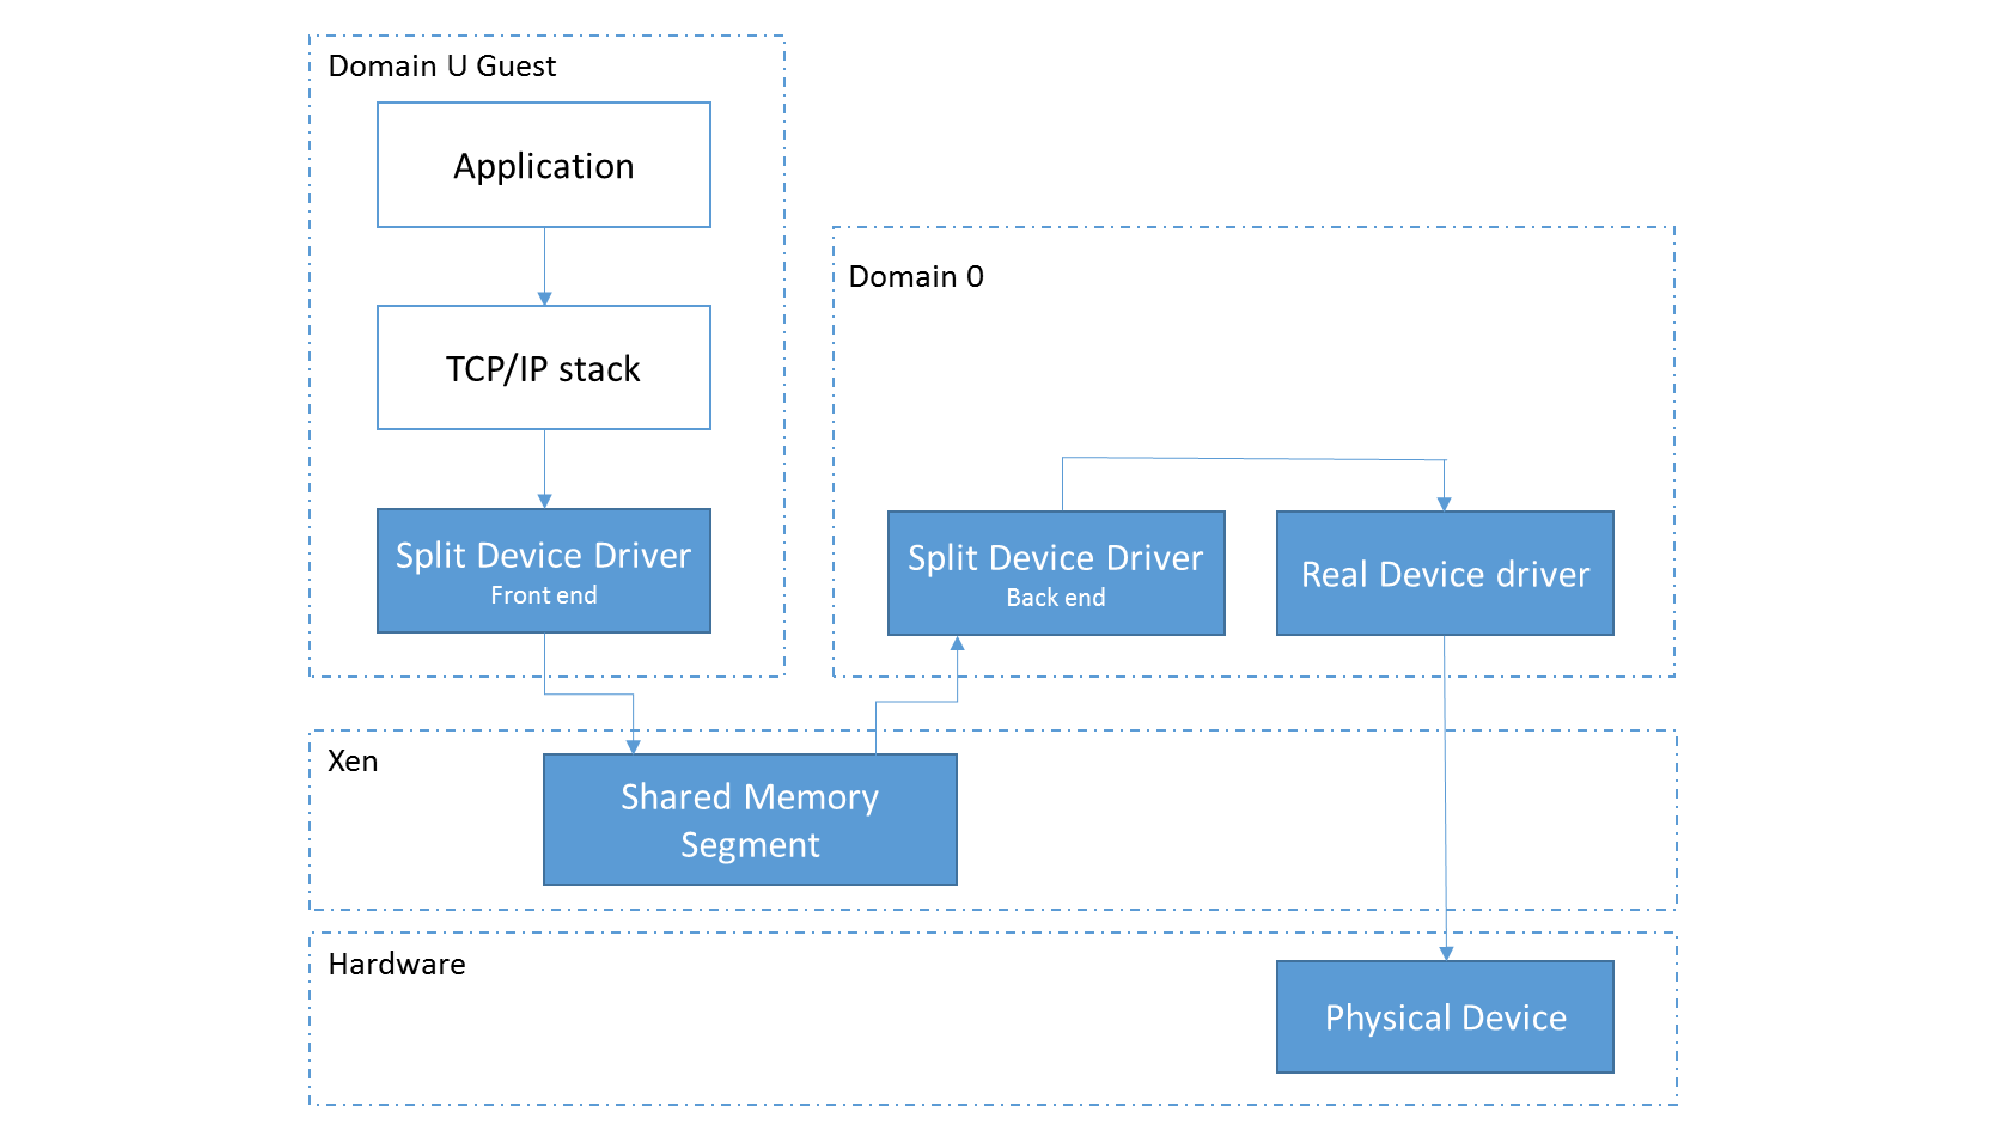
\includegraphics[scale=.50]{xen-split-tcp.pdf}
\caption{Split device driver model}
\label{fig:xen-split}
\end{figure}
Xen uses a frontend driver in the domains that wish to access the device
and a backend driver in the domain that runs the actual device driver. The
frontend and the backend drivers transfer data between domains over
a channel that is provided by the Xen virtual machine monitor (VMM).
Within the driver domain, the backend driver is used to demultiplex
incoming data to the device and to multiplex outgoing data between the
device and the guest domain~\cite{driverdomain}.

Isolated drivers use the same architecture, except that device drivers
do not execute in a single, privileged domain (Domain 0), but rather
a separate guest domain is created for each driver.
User applications and the kernel are executed in a separate domain.
As a result, device drivers are isolated from the 
kernel, making it impossible for the device driver to corrupt kernel
data structures in the virtual machine running user applications.

Despite advances in virtualization technology, the overhead of
communication between guest and driver domains significantly
affects the performance of applications~\cite{barham2003xen,
Sugerman:2001:VID:647055.715774, Menon:2006:ONV:1267359.1267361}. Isolated
driver domains follow an interrupt-based approach for sending
notifications~\cite{barham2003xen} between domains. The frontend and backend 
drivers notify each other of the receipt of a service request and corresponding responses
by sending an interrupt. The Xen hypervisor needs to schedule the
other domain to deliver the interrupt, which may require a context
switch~\cite{barham2003xen}. Such context switches can cause significant
overhead~\cite{Li:2007:QCC:1281700.1281702, Mogul:1991:ECS:106973.106982}.

\section {Proposed Solution}
\label{sec:solution}
In uniprocessor and multiprocessor environments, context switches may take
significant amounts of time. In a multiprocessor environment, it may be more
efficient for each process to keep its own CPU and spin while waiting
for a resource~\cite{Bovet:2005:ULK:1077084}. 

In this thesis, we propose and evaluate an optimization strategy
for improving the performance of the communication between guest and
driver domains. We propose a solution in which a thread in the backend
driver spins for some amount of time, checking for incoming service
requests. Similarly, the frontend driver spins while checking for
responses.  On multiprocessor environments, this solution performs better
than the interrupt-based approach used in the original implementation.

The source code of the isolated driver domain implementation as described 
by Fraser et al~\cite{driverdomain} is no longer available as part 
of the Xen hypervisor code distribution.  Therefore, we reimplemented isolated
driver domains; in this thesis, we refer to our implementation as IDDR
(Isolated Device Drivers). We implemented our spinning-based optimization 
within the IDDR framework.

We evaluated the performance of the IDDR system for multiple block device
types, including ramdisks, loop devices, and hard disks attached via 
the Serial Advanced Technology Attachment (SATA) interface standard. 
Each block device
is formatted with a ext2 file system and the IDDR system is evaluated
by measuring the performance of the system with the SysBench benchmark. 
The integrity of the system is checked by executing reads and writes on 
the block device, with and without read ahead, as well as by performing 
a number of file system tests on each block device type.  
Our evaluation showed that the performance
of the system can be improved by avoiding the context switches in
the communication channel and spinning instead. 
IDDR trades CPU cycles for better performance.  We believe this 
trade-off is acceptable particularly in multicore environments in 
which the CPU cycles used cannot easily be used by application code.

\section{Core Contributions}

The core contributions of this thesis are listed below: 
\begin{enumerate}
\item Reimplementation of isolated driver domains, referred to as IDDR.
\item Performance optimizations for IDDR by implementing a spinning-based 
        communication channel instead of an interrupt-based communication channel. 
\item Performance comparison of the spinning-based vs. interrupt-based approaches.
\end{enumerate}

\section {Organization}
This section provides the organization and roadmap of this thesis.

\begin{enumerate}
\item Chapter 2 provides background on processes, threads, memory protection, virtualization, hypervisors 
    and interdomain communication.
\item Chapter 3 provides an introduction to the design of the IDDR system.
\item Chapter 4 discusses the detailed design and implementation of IDDR. 
\item Chapter 5 evaluates the performance.
\item Chapter 6 reviews related work in the area of kernel fault tolerance.
\item Chapter 7 concludes the thesis and lists possible topics where this work can be extended.
\end{enumerate}

\pagebreak

\ifbool{toShowBibliography}{\bibliography{references}}{}
